\documentclass[a4paper,11pt,dvipdfmx]{jsarticle}


% 数式
\usepackage{amsmath,amsfonts}
\usepackage{bm}

% 画像
\usepackage[dvipdfmx]{graphicx}
\usepackage{framed}

% 図形
\usepackage{tikz}
\usetikzlibrary{shapes.geometric}
\usetikzlibrary {shapes.misc}

% ソースコード
\usepackage{listings,jlisting,color}
\lstset{
basicstyle={\ttfamily},
identifierstyle={\small},
commentstyle={\smallitshape},
keywordstyle={\small\bfseries},
ndkeywordstyle={\small},
stringstyle={\small\ttfamily},
frame={tb},
breaklines=true,
columns=[l]{fullflexible},
numbers=left,
xrightmargin=0zw,
xleftmargin=3zw,
numberstyle={\scriptsize},
stepnumber=1,
numbersep=1zw,
lineskip=-0.5ex
}
\renewcommand{\lstlistingname}{ソースコード}


\begin{document}
\definecolor{shadecolor}{gray}{0.70}

\title{画像処理 課題3 固有顔}
\author{21T2166D 渡辺大樹}
\date{\today}
\maketitle

\section{課題の目的・意図}
本課題では顔認識に関係する主成分分析(PCA)を用いた固有顔(EigenFaces)の生成を行い、その計算手順と結果を考察する。

\section{処理内容}
以下では固有顔の生成における処理内容について説明していく。

固有顔の生成は以下の手順で行う。
\begin{enumerate}
    \item 顔画像の前処理
    \item 顔画像の平均画像の算出
    \item 顔画像の共分散行列の算出
    \item 共分散行列の固有値分解
    \item 固有顔の生成
\end{enumerate}

\subsection{顔画像の前処理}
顔画像の前処理では、顔画像を読み込み、グレースケール化とOctaveでの処理のため、MAT形式化を行う。
今回、顔画像はインターネットよりダウンロードした証明写真のフリー素材と、生成AIを用いて生成した画像を用いた。入力画像は17枚とした。

これらの画像はそのままカラー画像として読み込むこともできたが今回はグレースケール化を行い、MAT形式で保存したのち処理をした。

この処理は固有顔の生成とは別ファイルで行った。演習とは無関係の処理のため生成AIを活用しながら作成したが、念のため\ref{mat}にそのコードを示す。

\subsection{顔画像の平均画像の算出}
顔画像の平均画像の算出では、前処理した顔画像を読み込み、データ行列を作成し、各画像の画素値を足し合わせ、画像数で割ることで平均画像を算出する。
データ行列は、各画像の画素値を行列の列として並べたものである。

例えば、$N$枚の画像があり、各画像の画素数が$M$であるとすると、データ行列$X$は$M \times N$の行列となる。

平均画像は、データ行列$\mathbf{X}$の各列の平均を取ることで得られる。この平均画像をデータ行列$\mathbf{X}$から引くことで、各画像の平均からの差分を取得することができる。
この平均画像を差し引いたデータ行列を$\overline{\mathbf{X}}$とする。

\begin{equation}
    \overline{\mathbf{X}} = \mathbf{X} - \mathbf{m}
\end{equation}

\subsection{顔画像の共分散行列の算出}
顔画像の共分散行列の算出では、平均画像を差し引いたデータ行列$\overline{\mathbf{X}}$を用いて、共分散行列$\mathbf{C}$を算出する。
共分散行列は、データ行列$\overline{\mathbf{X}}$の転置行列とデータ行列$\overline{\mathbf{X}}$の行列積をデータの個数で割ることで算出する。

\begin{equation}
    \mathbf{C} = \frac{1}{N} \overline{\mathbf{X}} \mathbf{X}^T
\end{equation}

共分散行列は、データの分散とデータ間の相関を表す行列であり、固有値分解を行うことで、データの主成分を求めることができる。

\subsection{共分散行列の固有値分解}
共分散行列の固有値分解では、共分散行列$\mathbf{C}$を固有値と固有ベクトルに分解する。
固有値と固有ベクトルは以下の式で表される。

\begin{equation}
    \mathbf{C} \mathbf{V} = \mathbf{D} \mathbf{V}
\end{equation}

ここで、$\mathbf{C}$は共分散行列、$\mathbf{V}$は各列が固有ベクトルである行列、$\mathbf{D}$は対角成分がそれぞれ固有値となる行列である。
すなわち、$\mathbf{V}$の一列目にあたる固有ベクトル$\mathbf{v_1}$と、$\mathbf{D}$の一列目にあたる固有値$\lambda_1$が対応する。

実際に固有値分解をする際は、共分散行列$\mathbf{C}$を固有値と固有ベクトルに分解する関数を用いることが一般的である。

\subsection{固有顔の生成}
固有顔の生成では、固有ベクトルを用いて、元の画像を固有顔に変換する。
まず、データ行列から平均画像を差し引いたデータ行列$\overline{\mathbf{X}}$と、固有ベクトル行列$\mathbf{V}$の積を取ることで、データの軸を標準基底に変換する。
続いて固有値行列$\mathbf{D}$を用いて、データの標準偏差を1にする。これは、固有ベクトルの長さを1にすることで、データの分散を1にすることに相当する。

この処理を行うことで、元の画像を固有顔に変換することができる。

\begin{equation}
    \mathbf{U} = \overline{\mathbf{X}} \mathbf{V} \mathbf{D}^{-\frac{1}{2}}
\end{equation}

\section{演習-考察}
以下では、固有顔の生成における演習結果について考察する。

\subsection{固有顔の生成}
まず、用いたデータセットの顔画像から16枚を図\ref{faces}に示す。

\begin{figure}[h]
\centering
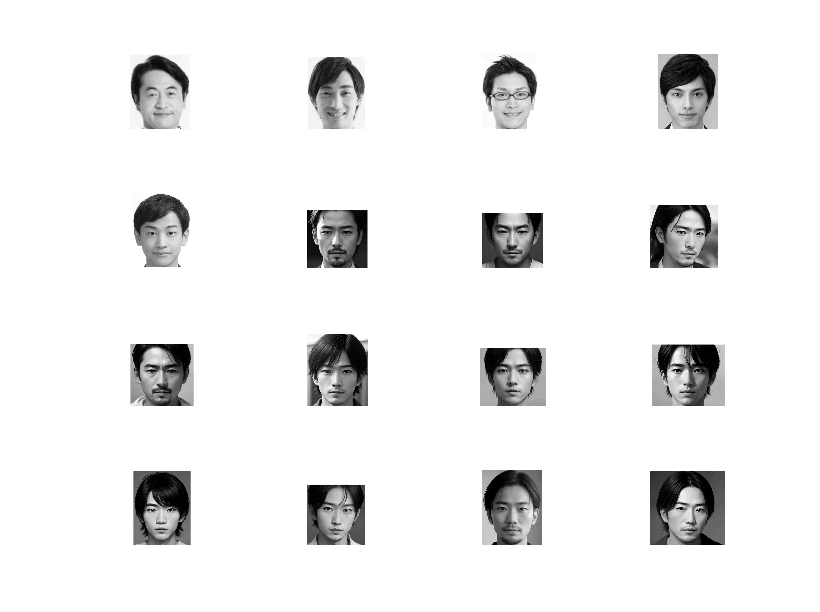
\includegraphics[width=100mm]{./img/figure.png}
\caption{顔画像}
\label{faces}
\end{figure}

生成AI特有の特徴がみられるデータセットとなっている。
\newpage

続いて、用意した顔画像17枚を用いて生成した固有顔の一部を図\ref{eigenfaces}に示す。

\begin{figure}[h]
\centering
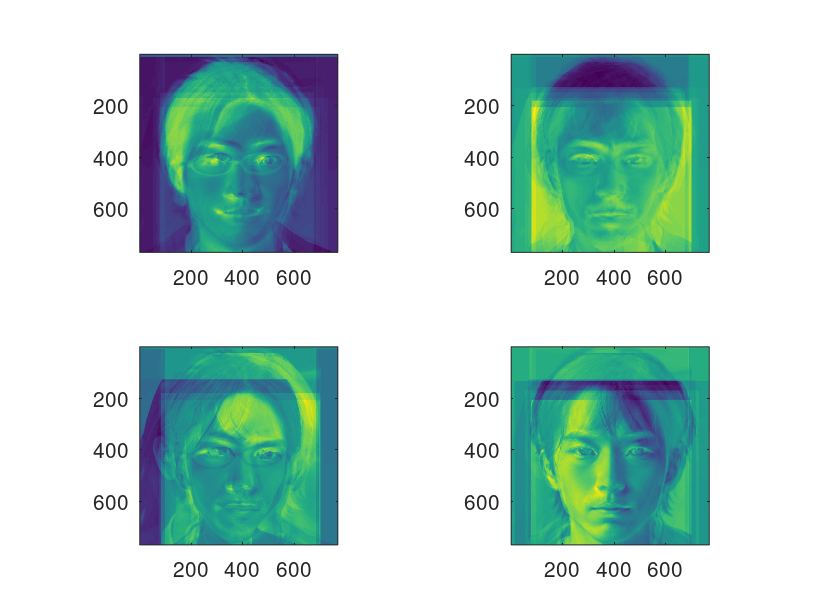
\includegraphics[width=100mm]{./img/figure2.png}
\caption{得られた固有顔}
\label{eigenfaces}
\end{figure}

データセットの特徴が反映された固有顔が得られていることがわかる。
また生成AI特有の顔つきが残る部分や、生成AIで出力されてしまい処理をしなかった背景が残る部分が特徴として出力されているのも読み取れる。
他にも目の位置のずれや、メガネなどの特徴が固有顔として出力されている。

\subsection{重みを用いた固有顔からの復元}
固有顔を用いれば、固有顔を生成したときと逆の計算で元の画像を復元することができる。

固有ベクトル行列$\mathbf{V}$の逆行列と固有値分解で得られた固有値の行列を$\frac{1}{2}$上したものの積を$\mathbf{W}$とする。
この$\mathbf{W}$を固有顔に掛け合わせ、平均画像を足すことで、元の画像データを復元することができる。

\begin{align}
    \mathbf{W} &= \mathbf{V} \mathbf{D}^{\frac{1}{2}} \\
    \mathbf{X} &= \mathbf{U} \mathbf{W} + m
\end{align}

この$\mathbf{W}$から任意のベクトルを選択することで、任意の元画像に変換することができる。

\begin{equation}
    \mathbf{x_1} = \mathbf{U} \mathbf{w_1} + m
\end{equation}

また、これを用いて、$\mathbf{W}$の任意のベクトルを重みをつけて足し合わせることで画像を合成することもできる。

\begin{equation}
    \mathbf{x} = \mathbf{U} (0.2\mathbf{w_1} + 0.8\mathbf{w_2}) + m
\end{equation}

この計算で生成される画像は、元の画像と異なる顔となる。

実際にこの計算を演習で行った結果を図\ref{reconstruction}に示す。

\begin{figure}[h]
\centering
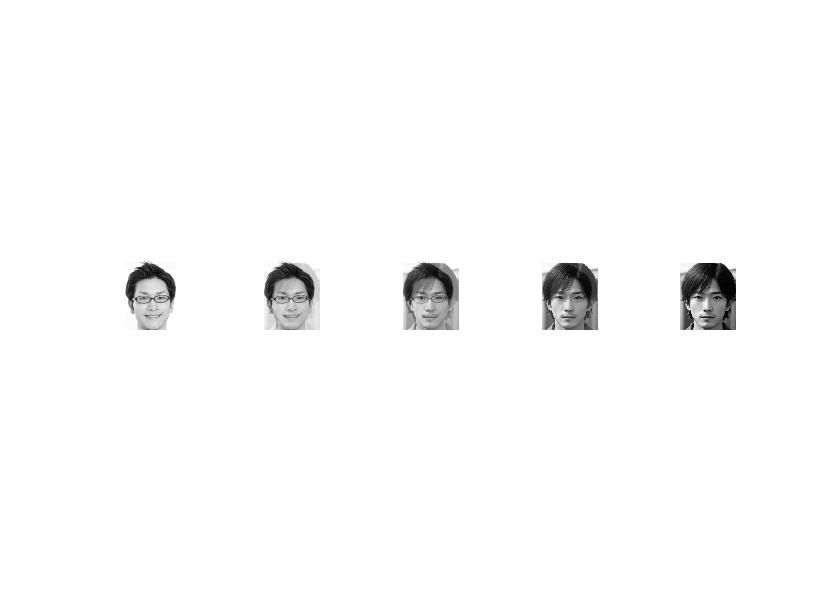
\includegraphics[width=100mm]{./img/figure5.png}
\caption{重みを用いた固有顔からの復元}
\label{reconstruction}
\end{figure}

この演習では重みを$S=[0, 0.2, 0.5, 0.8, 1]$と連続的に変化させて、
\begin{equation}
    \mathbf{x} = \mathbf{U} (S\mathbf{w_1} + (1-S)\mathbf{w_2}) + m
\end{equation}
として計算した。
実際にこの図\ref{reconstruction}のように、重みを変化させることで画像が連続的に変化しているのが分かる。

また重みが1や0となる部分では、$\mathbf{w}$に対応しているであろう元画像がそのまま復元されていることがわかる。

\section{実験に用いたコード}
以下に、実験に用いたコードを示す。

\lstinputlisting[caption={顔画像の前処理} label={mat}]{c:/Program_Code/Octave/task/mat.m}

\lstinputlisting[caption={固有顔の生成}]{c:/Program_Code/Octave/task/face.m}




\end{document}